\section{Ito chain rule}
\subsection{Formal derivation}
 We can write the discrete version of the SDE as:
 \begin{equation}
     \Delta x = A(x,t)\Delta t + B(x,t)\Delta W(t)
     \label{SDE}
 \end{equation}
 with the following conditions on $\Delta W$:
 \begin{equation}
     \begin{cases}
      \begin{aligned}
           & \langle \Delta W(t)\rangle = 0\\[2ex]
           & \langle \Delta W(t)\Delta W(t')\rangle = \delta_{t,t'}\Delta t
      \end{aligned}
     \end{cases}
 \end{equation}
 which enforce that the $\Delta W(t)$ are uncorrelated in time.\\
 We want now to find how to evolve this type of equation, that is we have $y(x)$ and we want to compute $\Delta y(x)$. We can expand $\Delta y(x)$ in series:
 \begin{equation}
 \begin{split}
     & y = y_0 + y'\Delta x + \frac{1}{2}y''\Delta x^2 + \frac{1}{6}y'''\Delta x^3 + \dots \\
     & \Delta y = y'\Delta x + \frac{1}{2}y''\Delta x^2 + \frac{1}{6}y'''\Delta x^3 + \dots 
 \end{split}
 \end{equation}
 and when $\Delta x$ is small we can keep only the terms up to the second order.\\
 We replace $\Delta x$ with Eq. \ref{SDE}, obtaining:
 \begin{equation}
     \Delta y = y'(A\Delta t + B\Delta W)+\frac{1}{2}y''(A^2\Delta t^2 + 2AB\Delta t\Delta W + B^2\Delta W^2) + \dots
 \end{equation}
 and we can check if some of the new terms are of an higher order than what we want to keep.\\
 Indeed we have that:
 \begin{equation}
     \begin{split}
         & A^2\Delta t^2 < A\Delta t\;\;for\;\;\Delta t\xrightarrow[]{} 0\\
         & 2AB\Delta t\Delta W < B\Delta W\;\;for\;\;\Delta t\xrightarrow[]{} 0
     \end{split}
 \end{equation}
 so we can neglect them.\\
 The remaining term ($B^2\Delta W^2 =B^2\Delta t R^2$) should be discarded on the basis that the power of $\Delta t$ is one and $R^2$ is a random number. Although we notice that we have $\langle R^2 \rangle = 1$, which means that the average contribution of this term is a drift, namely $B^2 \Delta t$. We can, then, keep just the term $B^2\Delta t$.\\
 Now we can write the equation that describes the evolution of $y(x)$, called \textbf{Ito chain rule}:
 \begin{equation}
 \Delta y = y'A(x,t)\Delta t + y'B(x,t)\Delta W + \frac{1}{2}y''B^2(x,t)\Delta t
     \label{Ito}
 \end{equation}
 we can see that the first two terms come from the classic chain rule, while the last is the one given by the stochastic nature of $x$.
 

 \subsection{Examples}
 
In this section we apply the Ito chain rule (Equation \ref{Ito}) to some practical examples: \\

\textbf{Example 1:} \begin{equation}
    dx = -xdt + dW \hspace{10mm} y = x^2
    \label{SDE_x_1}
\end{equation}

A numerical integration of the SDE on $x$ is the following:
\begin{figure}[H]
  \centering
  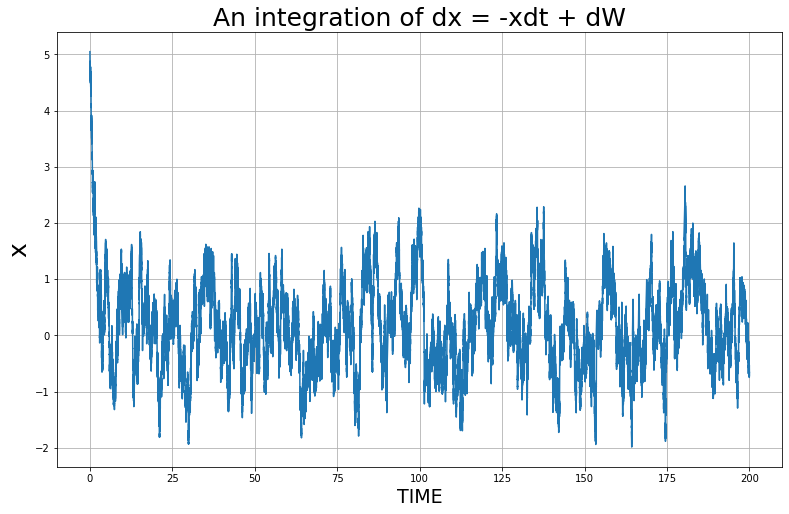
\includegraphics[width=0.8\textwidth]{SDE/Figures/SDEx.png}
  \caption{This numerical integration is produced using dt = 0.01, x(t=0) = 5, initializing the pseudo-random number generator with np.random.seed(1) and discarding the first element.} 
  \label{Fig:SDE_x_1}
\end{figure}

In this case we have:
 \begin{equation}
     \begin{split}
         & y' = 2x \\
         & y'' = 2 \\
         & A(x, t) = -x \\
         & B(x, t) = 1
     \end{split}
 \end{equation}

Applying Ito chain rule we get: 
  
\begin{align}
        \nonumber dy &= -2x^2dt + dt + 2xdW \\
        \nonumber &= (1-2x^2)dt + 2xdW\\
        \nonumber &= (1-2y)dt \pm 2\sqrt{y}dW\\
                  &= (1-2y)dt + 2\sqrt{y}dW
    \end{align}
\label{SDE_y_1}

Where in the last equation we used the fact that the plus and the minus sign generate the same SDE, since they are multiplied by an even random variable (i.e. gaussian random variable with zero mean).
We stress the fact that deriving a new SDE independent from $x$ (as in this case) is not always possible. \\
Equation (\ref{SDE_y_1}) might seem wrong because, if integrated with a finite time step $dt$, it can produce negative $y$'s, while we set $y = x^2$. This problem arises from the fact that we are using a finite time step. The smaller we set $dt$, the more it is unlikely to have negative $y$'s. So, instead of integrating Equation (\ref{SDE_y_1}), we simply square the values of Figure \ref{Fig:SDE_x_1} and produce the following figure: 
\begin{figure}[H]
  \centering
  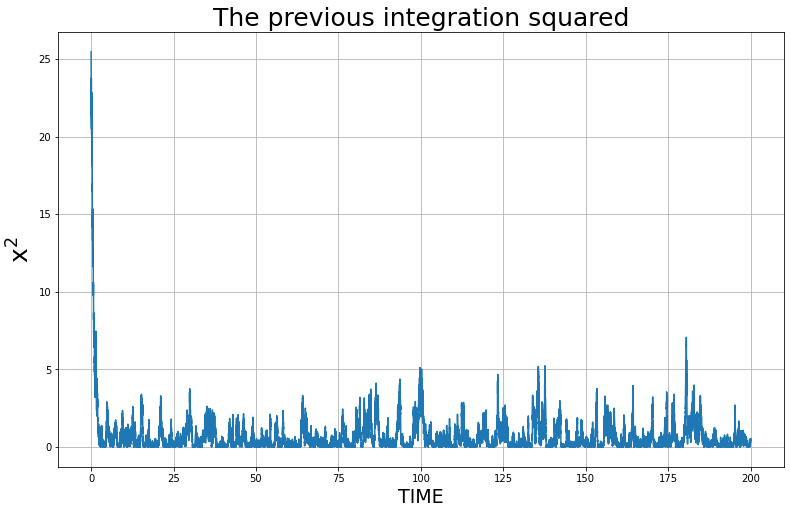
\includegraphics[width=0.8\textwidth]{SDE/Figures/SDEy.png}
  \caption{To produce this Figure we took the values in Figure \ref{Fig:SDE_x_1} and squared them.}
  \label{Fig:SDE_y}
\end{figure}

\textbf{Example 2:} 
\begin{equation}
    dx = BdW \hspace{10mm} y = e^x \hspace{10mm} B\hspace{1.5mm}constant
    \label{SDE_x_2}
\end{equation}
This is an example of Brownian motion/Random walk. 
3 numerical integrations of the same SDE on x are the following:
\begin{figure}[H]
  \centering
  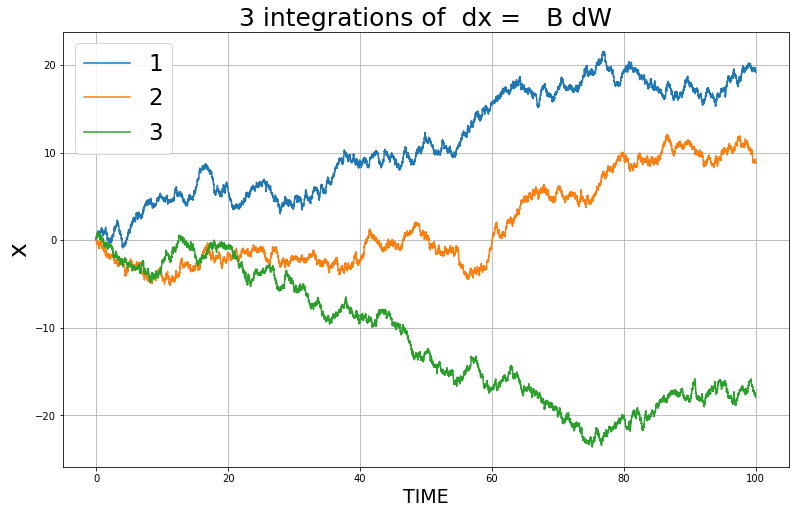
\includegraphics[width=0.8\textwidth]{SDE/Figures/SDEx_2.png}
  \caption{These numerical integrations are produced using dt = 0.01, x(t=0) = 0, initializing the pseudo-random number generator with np.random.seed(2) and discarding the first element.} 
  \label{Fig:SDE_x_2}
\end{figure}

In this case we have:
 \begin{equation}
     \begin{split}
         & y' = e^x = y \\
         & y'' = e^x = y \\
         & A(x, t) = 0 \\
         & B(x, t) = B
     \end{split}
 \end{equation}

Applying Ito chain rule we get: 
  
\begin{equation}
    dy = \frac{B^2y}{2}dt + BydW
    \label{SDE_y_2}
\end{equation}

It is worth noticing that, from Equation \ref{SDE_x_2}, we cannot expect $x$ to oscillate around a value as in the previous exercise (here there is only the random contribution). 

If we take the orange curve in Figure \ref{Fig:SDE_x_2} and apply the transformation y = $e^x$ we get:
\begin{figure}[H]
  \centering
  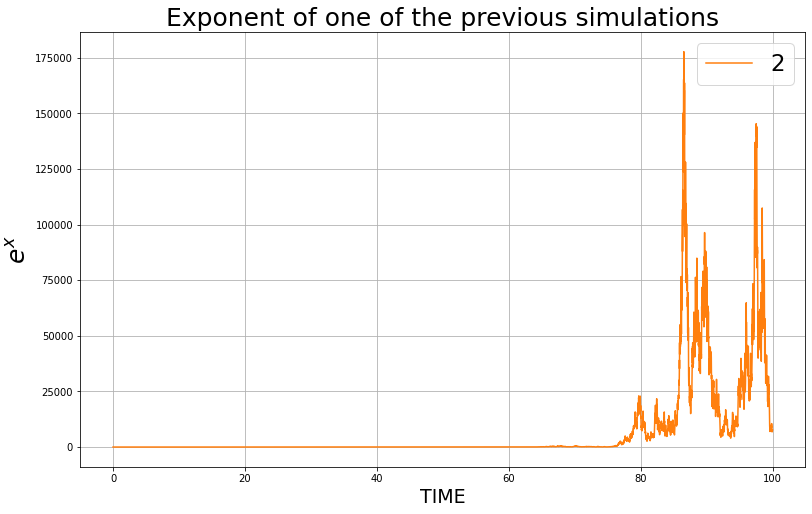
\includegraphics[width=0.8\textwidth]{SDE/Figures/SDEy_2.png}
  \caption{The exponent of each value of the orange simulation.}
  \label{Fig:SDE_x_2}
\end{figure}

\textbf{Example 3:} \begin{equation}
    dx_i = -x_i dt + dW_i \hspace{6mm} y = \sum_i x_i^2 \hspace{6mm} i = 1, ..., N
    \label{SDE_x_3}
\end{equation}

Defining $y_i$ = $x_i^2$ and  recalling Example 1 we write:
\begin{equation}
    dy_i = (1-2y_i)dt + 2\sqrt{y_i}dW_i
\end{equation}

Since $y$ is the sum of independent variables we can write:

\begin{align}
        \nonumber dy &= \sum_i dy_i = \sum_i (1-2y_i)dt + \sum_i 2\sqrt{y_i}dW_i \\
        \nonumber &= Ndt - 2\sum_i y_i dt + 2 \sum_i \sqrt{y_i}dW_i\\
        \nonumber &= Ndt - 2\sum_i y_i dt + 2 \sum_i \text{(Gaussian mean 0, variance $y_idt$)}\\
        \nonumber &= Ndt - 2y dt + 2\text{(Gaussian mean 0, variance $\sum_i y_idt$ = $ydt$)}\\
                  &= (N -2y) dt + 2\sqrt{y}dW
    \end{align}
\label{SDE_y_3}

We see that for N = 1 we recover the results of Exercise 1. \\

In this section we've always considered the random component to be normally distributed, but, in a stochastic process it could be possible to have different distributions that model the noise. In case of infinite variance we get discontinuity in the trajectory (the so-called Levy flights).


\subsection{Stratonovich formalism}
A stochastic differential equation can be represented also by using the so-called Stratonovich formalism, according to which
\begin{equation}\label{st}
\Delta x=A\Delta t+B(x+\frac{\Delta x}{2},t)\Delta W.
\end{equation}
As we can see from Eq. \eqref{st}, the random component $B$ is now evaluated in the middle point between the present position and the next position.

The same equation can therefore be expressed in two different ways depending on which formalism is used. In particular, we have
 \begin{align}
        \nonumber &dx=Adt+BdW \quad (\text{Ito})\\
        \nonumber &\dot{x}=A+B\eta \quad (\text{Stratonovich}),
    \end{align}
 where the coefficients $A,B$ are different for each formalism.
 
 

